\chapter{Gene Regulatory Networks}\label{grn}
\lhead[\fancyplain{}{\bfseries\thepage}]{\fancyplain{}{\bfseries\rightmark}}


\section{Definition}

Gene regulation controls the expression of genes and, consequently, all cellular functions. Gene expression is a process that involves transcription of the gene into mRNA, followed by translation to a protein, which may be subject to post-translational modification \cite{K40}. The transcription process is controlled by transcription factors (TFs) that can work as activators or inhibitors. TFs are themselves encoded by genes and subject to regulation, which altogether forms complex regulatory networks. 
\begin{figure}
\centering
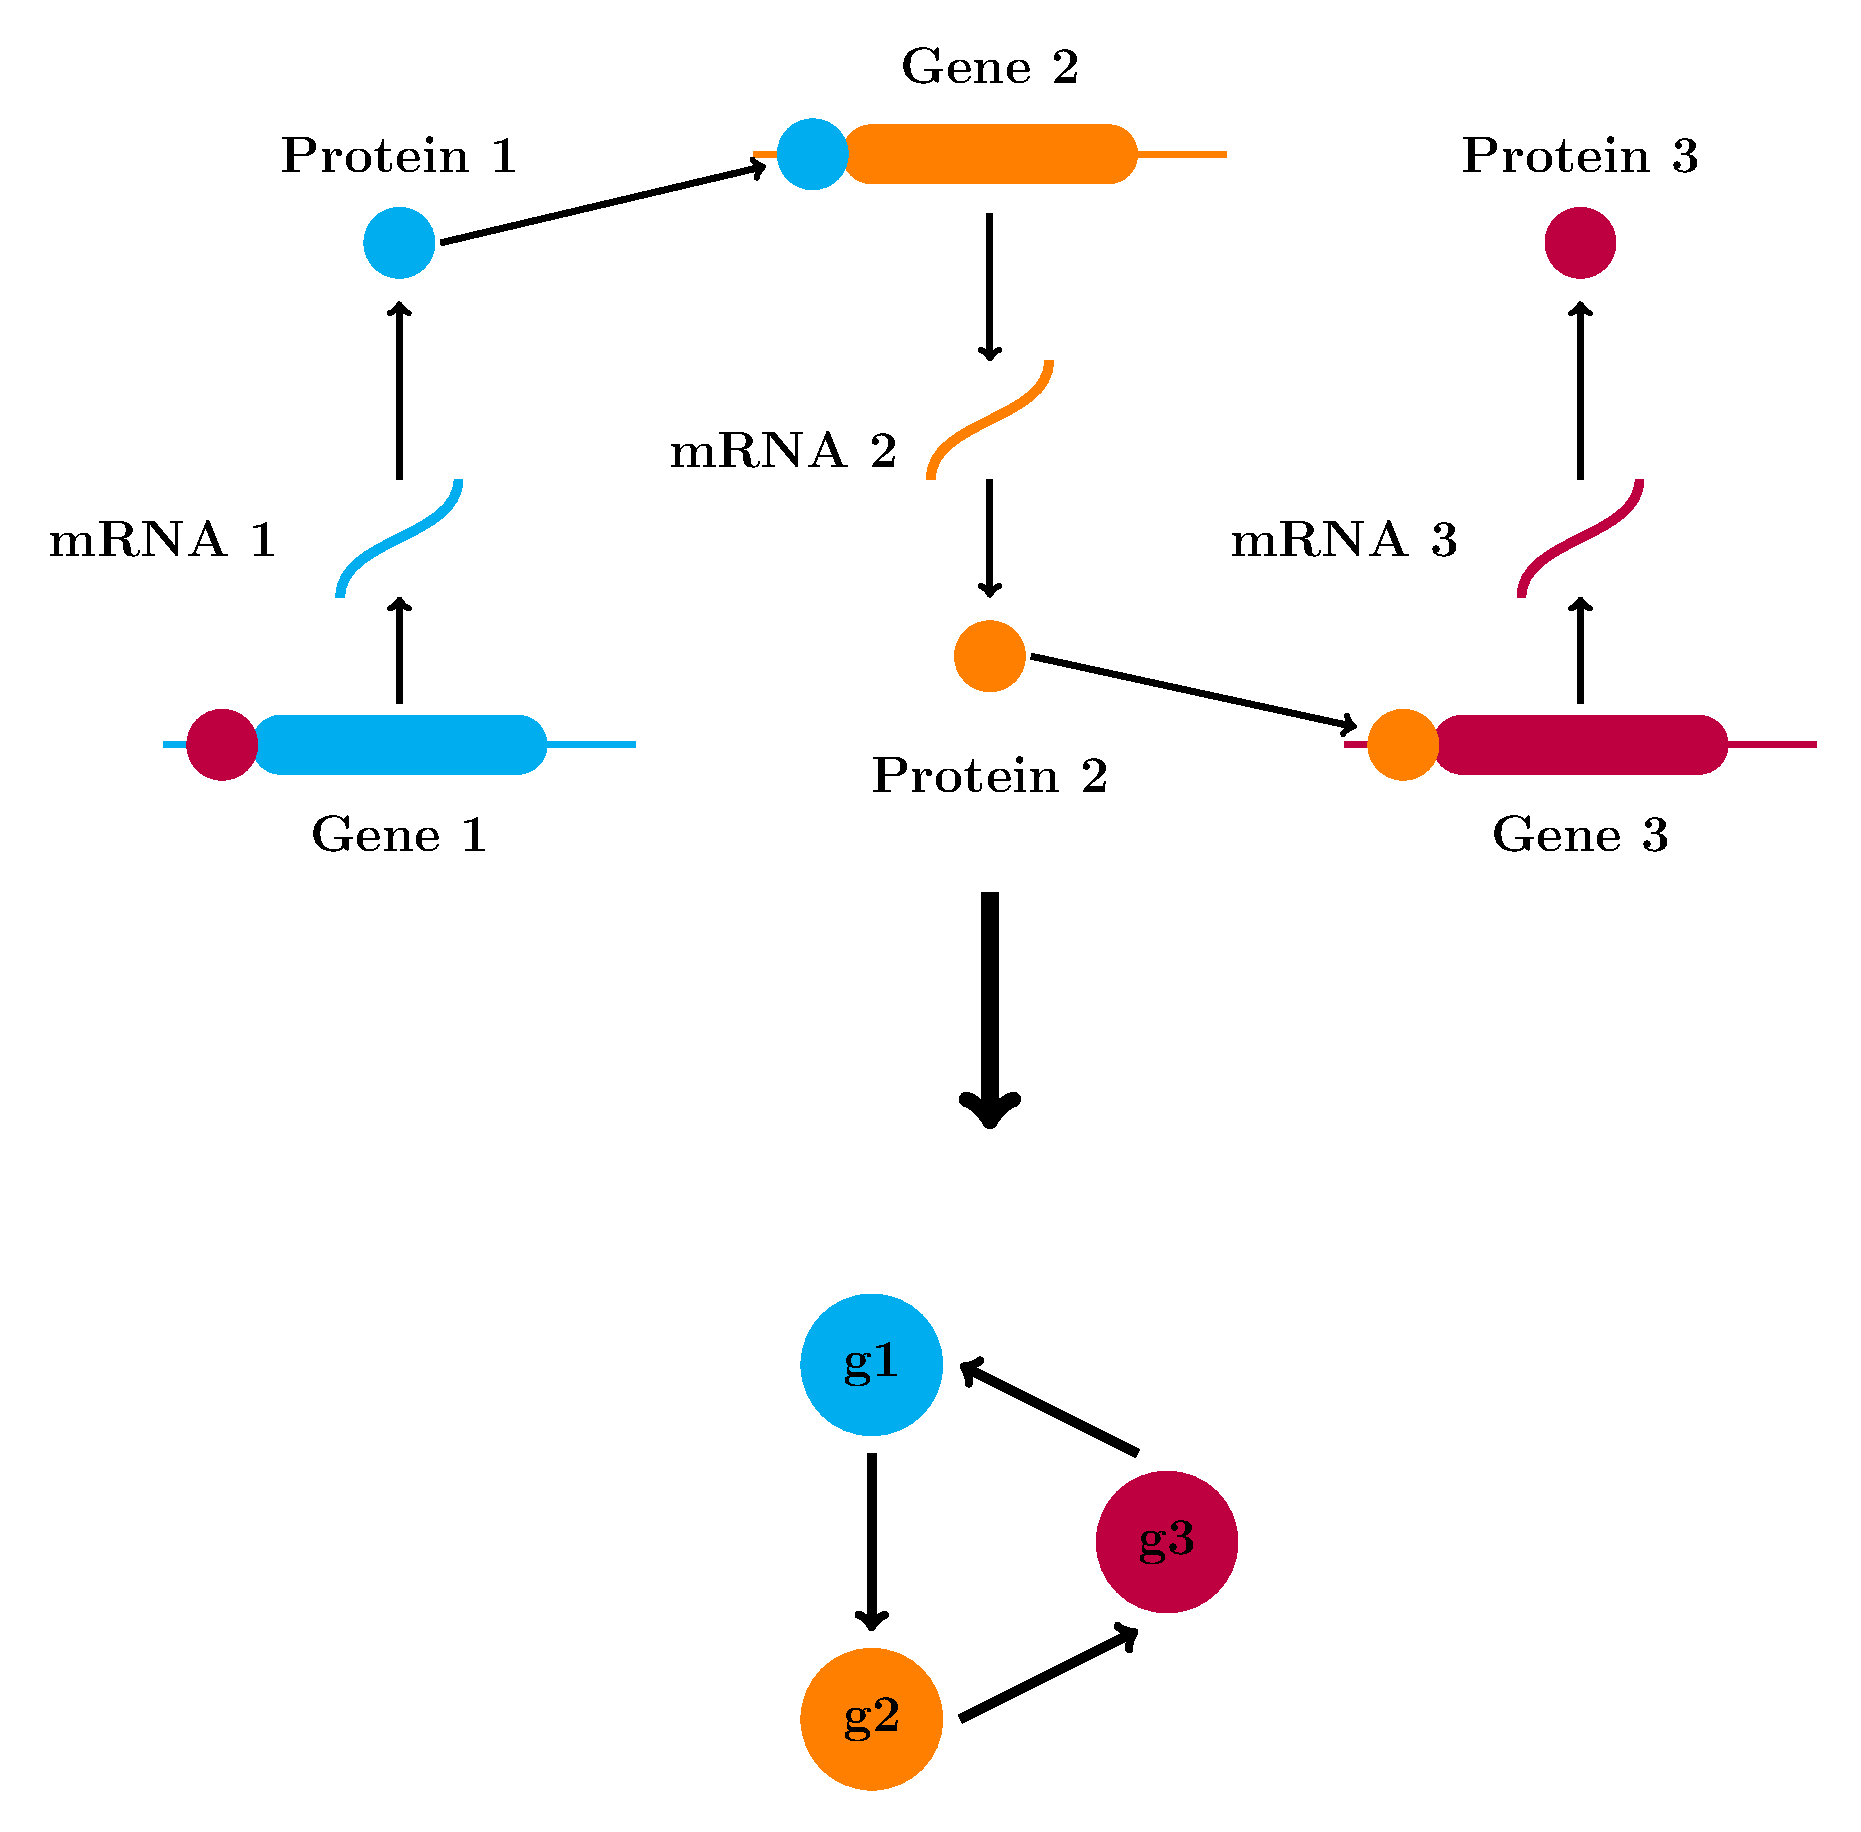
\includegraphics[scale=0.4]{images/grnn.pdf}
\caption{\emph{Schematic representation of a Gene Regulatory Network.}}
\end{figure}
Cells efficiently carry out molecular synthesis, energy transduction, and signal processing across a range of environmental conditions by networks of genes, which we define broadly as networks of interacting genes, proteins, and metabolites \cite{K37}. Formally speaking, a \emph{gene regulatory network} or \emph{genetic regulatory network} (GRN) is a collection of DNA segments in a cell which interact with each other (indirectly through their RNA and protein expression products) and with other substances in the cell, thereby governing the rates at which genes in the network are transcribed into mRNA. In general, each mRNA molecule goes on to make a specific protein (or set of proteins). In some cases this protein will be structural, and will accumulate at the cell-wall or within the cell to give it particular structural properties. 

These networks control biological process of all organisms. The complex control systems underlying development have probably been evolving for more than a billion years. They regulate the expression of thousand of genes in any given biological process. They are essentially hardwired genomic regulatory codes, the role of which is to specify the sets of genes that must be expressed in specific spatial and temporal patterns. In physical terms, these control system consist of many thousands of modular DNA sequences. Each module receives and integrates multiple inputs, in the form of regulatory proteins (\emph{activators} and \emph{repressors}) that recognize specific sequences within them. The end result is the precise transcriptional control of the associated genes. 
Functional linkages between these particular genes, and their associated regulatory modules, define the core networks underlying development. They explain exactly how genomic sequence encodes the regulation of expression of the sets of genes that generate patterns and execute the construction of multiple states of differentiation.

The regulatory genome is a logic processing system: every regulatory module contained in the genome receives multiple inputs and processes in ways that can be mathematically represented as combinations of logic functions. 

Definitive regulatory functions emerge only from the architecture of intergenic linkages, and these functions are not visible at the level of any individual genes. So gene regulatory networks can be determined only by experimental molecular biology in which the functional meaning of given regulatory sequences is directly determined.

GRNs have a complex structure: they are inhomogeneous compositions of different kinds of subnetworks, each performing a specific kind of function. Some subnetworks are used in many processes.

In principle, mathematical modeling of GRN dynamics can provide a theoretical foundation for understanding cell heterogeneity and gene expression dynamics, by quantitatively linking molecular-level regulatory mechanisms with observed cell states. However, due to the molecular complexity of gene regulatory mechanisms, it remains challenging to integrate such models with single-cell data.

\section{Modelling GRNs}
Mathematical models can account for (and at least partially reproduce) observed cellular heterogeneity in two primary ways. First, gene network models are multistable dynamical systems, meaning a given network has the potential to reach multiple stable states of gene expression. These states arise from the dynamic interplay of activation, inhibition, feedback, and nonlinearity \cite{K1} \cite{K42}. Second, some mathematical models inherently treat cellular noise. This noise, or stochasticity, is modeled in various ways depending on assumptions about the source \cite{K43} \cite{K44}. Discrete, stochastic models of gene regulation, which track discrete molecular entities, regulatory-protein binding kinetics, and binding states of promoters controlling gene activity, have formed the basis of biophysical theories of gene expression noise due to so-called intrinsic molecular noise \cite{K44} \cite{K45}. Such stochastic gene regulation mechanisms have also been incorporated into larger regulatory network models using the formalism of stochastic biochemical reaction networks, and have been utilized to explore how molecular fluctuations can cause heterogeneity within phenotype-states and promote stochastic transitions between phenotypes \cite{K46} \cite{K47}.

The quantitative landscape of cellular states is another concept that is increasingly utilized to describe cellular heterogeneity. Broadly, the cellular potential landscape (first conceptualized by Waddington \cite{K12}\cite{K13}) is a function in high-dimensional space (over many molecular observables, typically expression levels of different genes), that quantifies the stability of a given cell state. In analogy to potential energy (gravitational, chemical, electric, etc.), cell states of higher potential are less stable than those of lower potential. The landscape concept inherently accounts for cellular heterogeneity, since it holds that a continuum of states is theoretically accessible to the cell, with low-potential states (in “valleys”) more likely to be observed than high-potential states. The landscape is a rigorously defined function derived from the dynamics of the underlying gene network model, according to some choice of mathematical formalism \cite{K48}\cite{K12}. 

Stochastic modeling of gene network dynamics has been employed in various forms for analysis of single cell measurements. However, few existing analysis methods utilize discrete-molecule, stochastic models, which fully account for intrinsic gene expression noise and its impact on cell-state, to aid in the interpretation of noisy distributions recovered from single cell RNA sequencing data \cite{K10}\cite{K11}. There exists an opportunity to link such biophysical, stochastic models, which reproduce intrinsic noise and cell heterogeneity in silico, to single cell datasets that characterize cell heterogeneity in vivo. In particular, the landscape of heterogeneous cell states computed from discrete stochastic models can be directly compared to single-cell measurements.

\section{Principle of the models}
GRNs may be interpreted as an idealized dynamical system of
model genes with directional links (transcription factors), updating
their state in parallel, according to the combinatorial logic of their
inputs, Kauffman's Random Boolean Networks \cite{K1}\cite{K7}.
There is justified debate as to whether parallel (synchronous) updating,
and the on-off characterization of genes, are valid idealizations when applied
to real genomic networks, given that transcription is asynchronous and driven
at different rates. However, gene activity at the molecular scale consists of
discrete events occurring concurrently. Variable protein concentrations can be
accounted for by genes being on for some fraction of a given time span. The
RBN idealization is arguably a valid starting point for gaining insights into
gene network dynamics.
In a cell type's gene expression pattern over a span of time (i.e. its space-
time pattern), a particular gene may, broadly speaking, be either on, off, or
changing. If a large proportion of the genes are changing, chaotic dynamics, the cell will be unstable. On the other hand, dynamics that settles to
a pattern where a large proportion of the genes are permanently on or o
(frozen) may be too in exible for adaptive behavior. Cells constantly need to
adapt their gene expression pattern in response to a variety of hormone and
growth/di erentiation factors from nearby cells. The definition of a cell type
may be more correctly expressed as a set of closely related gene expression
patterns, allowing an essential measure of exibility in behavior.

In the next Chapter we will concentrate on the Random Boolean Networks proposed by Kauffmann in 1969.
